\section{Data}
\subsection{Description the data}
\noindent
\par The data we are using can be found on the OpenfMRI website at the following
address: \url{https://www.openfmri.org/dataset/ds000005}, the dsnum is ds005.
For our project, we are specifically using the behavior data and the BOLD data
that are organized. 

\noindent
\par For each of runs per subject (3), the behavior data contains the timestamp of
each survey question (onset), the gain/loss combinations (gain and loss), the
response for the particular trial (respnum) from the 4-point likert scale. 
The researcher created a response category (respcat) to be used in their binary
choice model that combines the “reject” answers together on one hand and the 
“accept” answers together on the other hand. BOLD data contains compressed  
4-dimensional brain images for each subject’s run. The folder also comports
Quality Assurance (QA) files and a report.

\noindent
\par Thanks to the resampling method and templates made made available by the 
the Montreal Neurological Institute, filtered have also been provided. 
The files have been resampled to a normalized 2mm voxel sizes. This standardization
method of the brain will allow us to perform cross subject or cross run analyses.

\subsection{Exploratory Analysis}

\noindent
We explore the data by reproducing some provided figures from the QA report and 
provided by the OpenfMRI researchers. The Figures \ref{fig:moisaic1} and 
\ref{fig:moisaic2} show the transversal slices of brain images with the mean values 
of the voxels accross time.

\begin{figure}[H]
\begin{subfigure}{.5\textwidth}
  \centering
  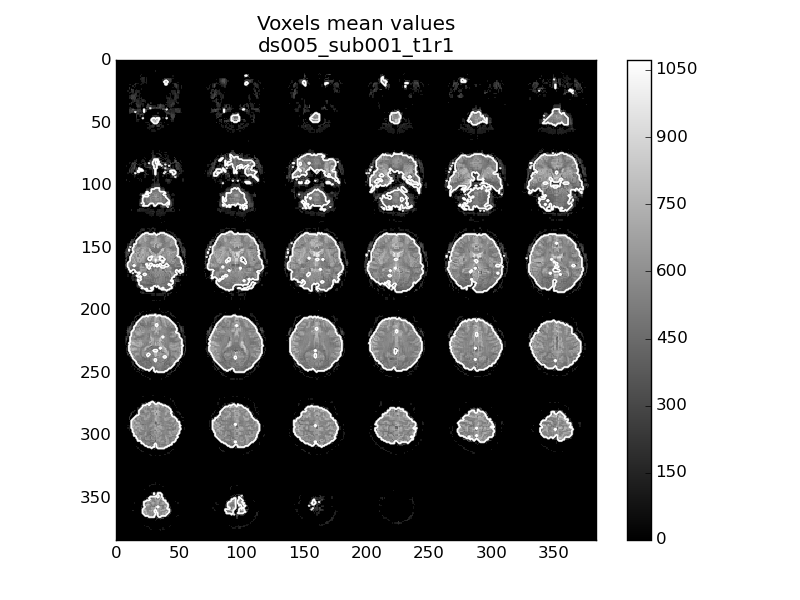
\includegraphics[width=.95\linewidth]{../fig/BOLD/ds005_sub001_t1r1_mean_voxels.png}
  \caption{Subject 1}
  \label{fig:mosaic1a}
\end{subfigure}%
\begin{subfigure}{.5\textwidth}
  \centering
  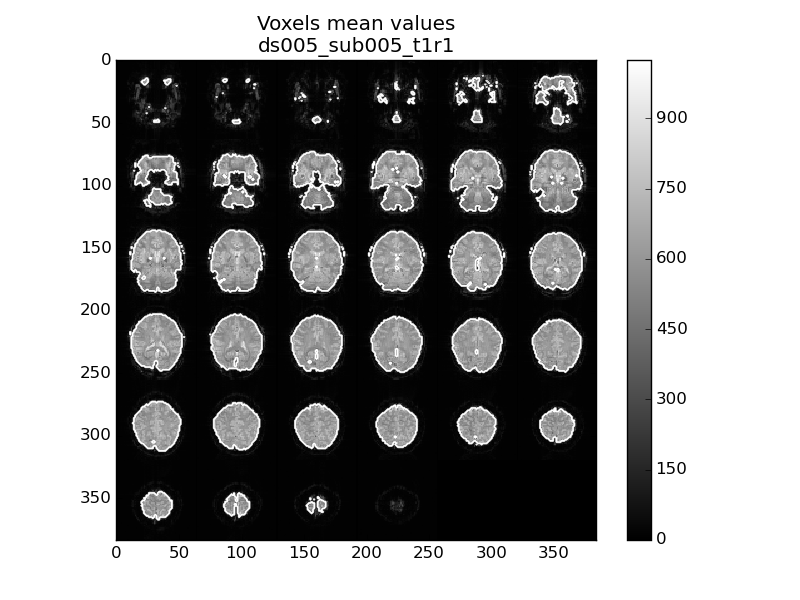
\includegraphics[width=.95\linewidth]{../fig/BOLD/ds005_sub005_t1r1_mean_voxels.png}
  \caption{Subject 5}
  \label{fig:mosaic1b}
\end{subfigure}
\caption{Mean value of the voxels accross time for the 34 slices of the transveral cut
         of the brain raw data for subject 1 and subject 5}
\label{fig:moisaic1}
\end{figure}

\begin{figure}[H]
\begin{subfigure}{.5\textwidth}
  \centering
  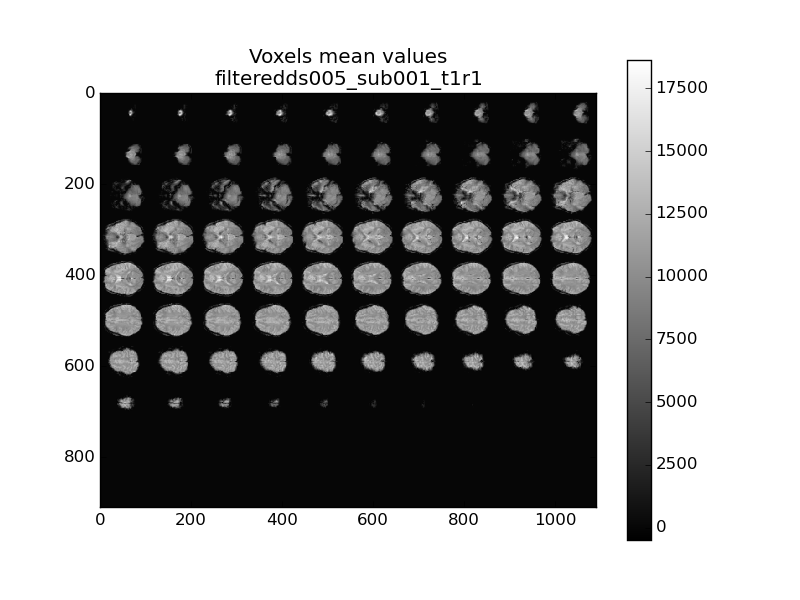
\includegraphics[width=.9\linewidth]{../fig/BOLD/filteredds005_sub001_t1r1_mean_voxels.png}
  \caption{Subject 1}
  \label{fig:mosaic2a}
\end{subfigure}%
\begin{subfigure}{.5\textwidth}
  \centering
  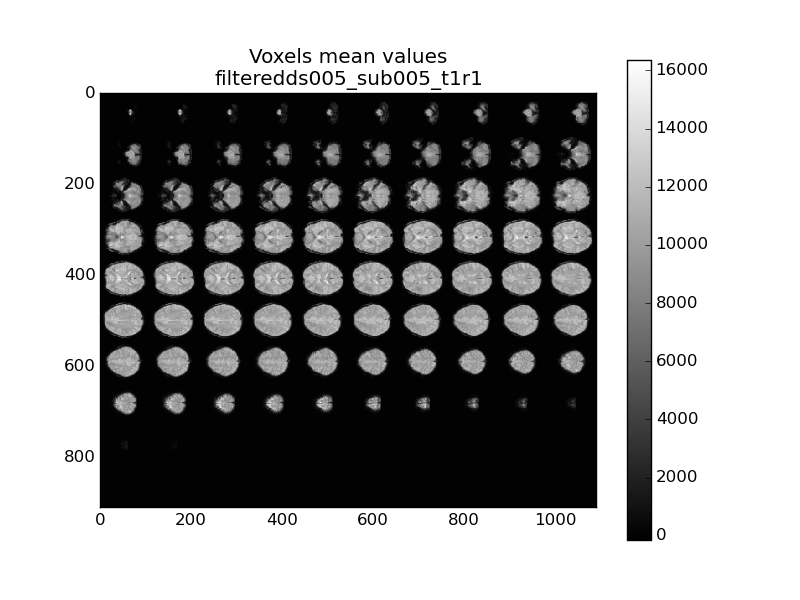
\includegraphics[width=.9\linewidth]{../fig/BOLD/filteredds005_sub005_t1r1_mean_voxels.png}
  \caption{Subject 5}
  \label{fig:mosaic2b}
\end{subfigure}
\caption{Mean value of the voxels accross time for the 91 slices of the transveral cut
         of the brain filtered data for subject 1 and subject 5}
\label{fig:moisaic2}
\end{figure}

\noindent
\par In Figure \ref{fig:rms}, we visualize the root mean square difference across
time between for the 1rst run of subecjt 1 and 5. 
As we expected, there is variations in the voxels volumes accross time. The noise 
correction is addressed in the BOLD image analysis section. These graphs also show that
there is a big difference in 'mean brain activation' accross subject. We will explore these
differences that can be tied to behavioral data as seen in the next section.

\begin{figure}[H]
\begin{subfigure}{.5\textwidth}
  \centering
  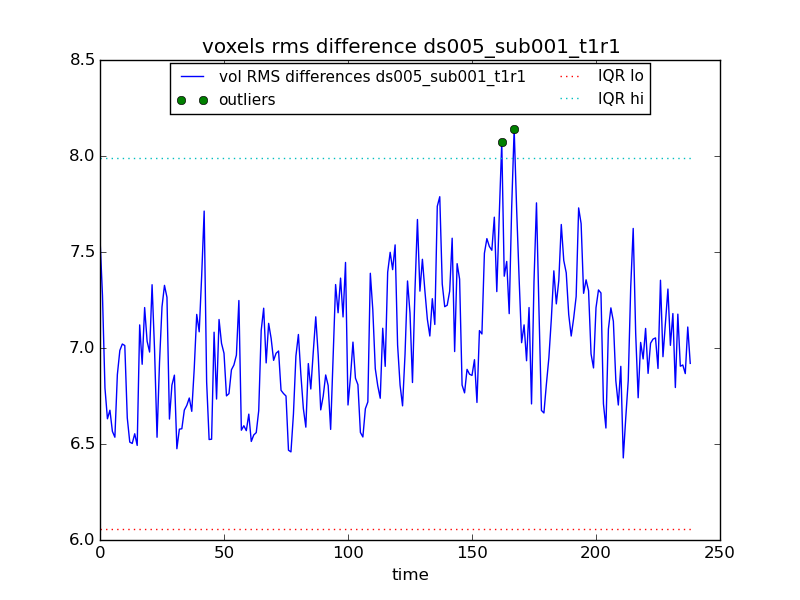
\includegraphics[width=.9\linewidth]{../fig/outliers/ds005_sub001_t1r1_vol_rms_outliers.png}
  \caption{Subject 1}
  \label{fig:rmsa}
\end{subfigure}%
\begin{subfigure}{.5\textwidth}
  \centering
  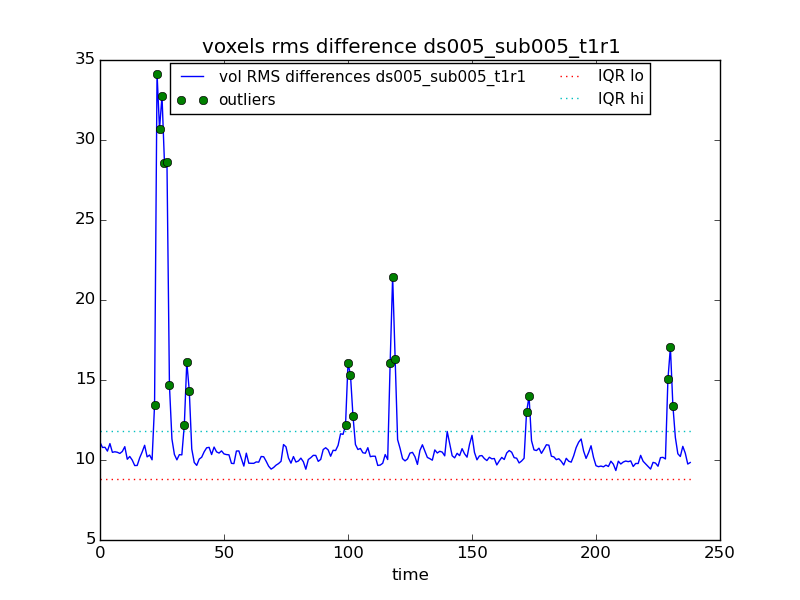
\includegraphics[width=.9\linewidth]{../fig/outliers/ds005_sub005_t1r1_vol_rms_outliers.png}
  \caption{Subject 5}
  \label{fig:rmsb}
\end{subfigure}
\caption{Voxels time course root mean square for subject 1 and 5 - run 1}
\label{fig:rms}
\end{figure}
